\chapter{The state-of-the-art of bilayer heterostructure of $MoS_2/WS_2$}

\section{Introduction}

As two-dimensional TMDCs have emerged as promising candidate materials for next-generation electronic and optoelectronic technologies with valley functionalities it has become apparent the need of enhancing some of their properties in view of their applications. For instance, creating band offsets between different monolayer TMDCs would enable efficient separation of charge carriers and rectification of charge flow. This would offer a mechanism for designing devices made by entirely van der Waals atomically thin materials.  Furthermore, the semiconducting monolayer TMDCs — $MoS_2$, $MoSe_2$, $WS_2$ and $WSe_2$ — are also interesting because they possess direct bandgap in the visible region at energy degenerate band edges (valleys), spin–valley coupling and valley-contrasting electronic and excitonic properties.
 The valley physics of TMDC excitons have been intensely studied in the past few years, with recent advances including the optical generation and control of exciton valley coherence. However, as the valley degree of freedom is affected by very fast recombination time (picosecond timescale) would impede any possible exploitation of the valley-functional optoelectronic devices based on valley excitons in monolayer TMDCs in practical applications. The fabrication of bilayered van der Waals (vdW) heterostructures would enable to fully exploit the potential of TMDC in electronic, opto and valleytronic applications.

\section{Properties of bilayer heterostructures}

As it has been explained in Chapter 1, TMDs undergo a crossover from indirect bandgap in the bulk to direct bandgap in the monolayer form. As a consequence of this direct band gap, monolayers absorb and emit light rather efficiently. The band structure changes as a function of the number of layers due to the strong interlayer coupling, which results in different shifts in the conduction and valence band edges at various symmetry points in the Brillouin zone as a function of the layer number.  Vertical sTMDs heterostructures formed by stacking up different monolayers offer a rich collection of physics and functionalities. Theory predicts that any stacked $MX_2$ heterostructures form type II semiconductor heterojunctions and thus it facilitate efficient electron–hole separation. This would be particularly beneficial for light harvesting and light detection applications. It has been further demonstrated that the charge separation can occurs over ultra fast time scales, such as femtosecond \cite{Hong2014}.
In type II semiconductor heterojunctions, the conduction band minimum and valence band maximum are found in two separate materials. If electrons and holes are photoexcited they will then prefer to stay in different materials. The alignment of electronic bands of $MoS_2$ and $WS_2$ monolayers as predicted \cite{Gong2013} is reported in Figure \ref{fig:HeterostructuresChargeSeperationDiagram}. It shows that monolayer $MoS_2$ and $WS_2$ have bandgaps of ~2.39 eV and ~2.31 eV, respectively, and the $MoS_2$ valence band maximum is 350 meV lower than that of $WS_2$ and the conduction band level is also lower. Thus is this material system, the conduction band minimum resides in $MoS_2$ and the valence band maximum in $WS_2$. This heterojunction structure can lead to efficient charge transfer upon optical excitation with separated electrons and holes residing in two layers. Hong et al has demonstrated that the electron-hole separation occurs in ~50 fs. The fast separation can be particular beneficial in solar-driven applications such as photoelectron catalysis and solar cells as it reduces the chances of immediate recombination of the charges.
We have demonstrated that the formation of this type of heterojunction of chemically exfoliated $MoS_2$/$WS_2$ and assembled in a form of thin films can be beneficial for photoelectrochemical water splitting. In Chapter \ref{cha:Heterostructures} we discuss the formation of $MoS_2$/$WS_2$ heterostructures in the form of thin films via CVD and their identification via physical characterization. The same structures have been used for photoelectrochemical water splitting. In general, the most studied bilayer heterostructures is formed by $MoS_2$ and $WS_2$ monolayers. This is due to the fact that synthesis of these materials via CVD is better established as compared to the selenides materials. 

\begin{figure}[h]
	\begin{center}
		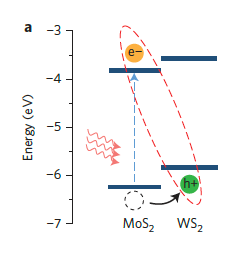
\includegraphics[scale=1]{Heterostructures/HeterostructureChargeSeparationDiagram.png}
		\caption{Charge seperation across heterojunction following photoabsorption}
		\label{fig:HeterostructuresChargeSeperationDiagram}
	\end{center}
\end{figure}

\section{Fabrication of bilayer heterostructures}

The first studies of heterostructures of TMDCs have been based on CVD materials. Two different approaches have been adopted. The first strategy was based on the transfer of two monolayers priorly synthesized independently.  While the second approach, which has not seen nearly any further work on, was based on the direct synthesis of heterostructures via CVD. 

\subsubsection{Transfer -approach}

$WS_2$/$MoS_2$ heterostructures have been prepared from conventional PDMS stamping method from CVD grown monolayers \cite{Tongay2014}. In the first report about this \cite{Gong2014}, $MoS_2$ and $WS_2$ monolayers have been grown by high-pressure CVD technique onto $SiO_2/Si$ substrates. The CVD $MoS_2$ monolayers were continuous over 1mm with large, single-domain crystals reaching up to 75 microns while the CVD $WS_2$ monolayers were in the form of individual triangle islands of ~5-50 microns in size. 
The fabrication process consisted in a first transfer of the WS2 monolayers onto PDMS substrates, followed by stamping the WS2 monolayers onto CVD $MoS_2$ monolayers, which formed vertical heterostructures of $WS_2$/$MoS_2$ \cite{Tongay2014}. The overlap region (approximately 40 ${\mu}m$) of $MoS_2$ and $WS_2$ monolayers show slightly darker contrast under the optical microscope and it is the region which has been characterized by Raman spectroscopy and photoluminescence and electrical measurements.

\begin{figure}[h]
	\begin{center}
		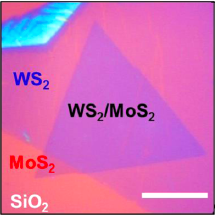
\includegraphics[scale=1]{Heterostructures/HeterostructureOpticalMap.png}
		\caption{Optical micrograph of the heterostructure of $WS_2$/$MoS_2$}
		\label{fig:HeterostructuresOpticalMap}
	\end{center}
\end{figure}

\subsubsection{Direct synthesis of vertical heterostructures}

Firstly, with the term, vertical heterostructures, we differentiate those from the lateral heterojunction created by two adjacent and consecutive layers of two different TMDs.
This terminology differentiates these two different types of heterojunction which can be obtained by direct CVD synthesis.
The direct synthesis of bilayer heterostructures have been obtained via CVD where molybdenum trioxide ($MoO_3$) powder was placed in  front of a bare $SiO_2/Si$ wafer for the growth of $MoS_2$ in a tubular furnace. A mixed powder of tungsten and tellurium was scattered on the wafer for the growth of $WS_2$. A small amount of tellurium was used to accelerate the melting of tungsten powder during the growth \cite{Gong2014}. Upstream in a low-temperature zone, the sulphur powder was placed. The furnace was heated up to the temperature range of 650-850 {\degree}C and argon gas was used as a carrier gas to protect the system from oxygen and carry sulphur vapour from the upstream of the tube during the reaction. The difference in the nucleation and growth rates of $MoS_2$ and $WS_2$ and the chosen growth temperature favours the sequential growth of $MoS_2$ and $WS_2$, instead of  the formation of their ternary alloy ($Mo_xW_{1-x}S_2$ alloy). Vertically stacked bilayers were found to grow preferentially at temperature of ~850 {\degree}C, whereas in-plane lateral heterojunctions were found at ~650 {\degree}C. The CVD  synthesis can lead to clean interfaces \cite{Gong2014}[our paper submitted ] between the two monolayer components, in contrast with mechanical transfer of layers or assembly from liquid phase. A typical optical, SEM and atomic force microscopy (AFM) images of the layers are shown in Figure \ref{fig:HeterostructuresOpticalSEMAFMImages}. The bilayers can be easily distinguished from monolayers via optical contrast (Figure \ref{fig:HeterostructuresOpticalSEMAFMImages}), with $MoS_2$ monolayers showing a light purple colour and the bilayer regions a much darker purple.

\begin{figure}[h]
	\begin{center}
		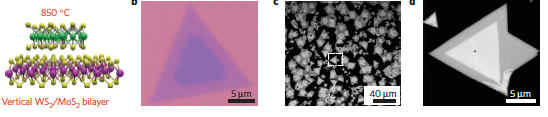
\includegraphics[scale=1]{Heterostructures/HeterostructureOpticalSEMAFMImages.png}
		\caption{Heterostructure imaging}
		\label{fig:HeterostructuresOpticalSEMAFMImages}
	\end{center}
\end{figure}

\section{Characterization of bilayer heterostructures}

\subsection{Raman spectroscopy}

Heterostructures fabricated by both these approaches were characterized by Raman spectroscopy. As the vibrational modes of $MoS_2$ and $WS_2$ are quite different the Raman spectrum of the heterostructure displays in-plane ($E^1_{2g}$) and out-of-plane ($A_{1g}$) modes of MoS2 and WS2 at the same frequencies as in their monolayers. The $WS_2$ $E^1_{2g}$ and $A_{1g}$ modes are located at 350 $cm^{-1}$ and 416 $cm^{-1}$ while for $MoS_2$ they are at 380 $cm^{-1}$ and 405 $cm^{-1}$ respectively. Spatial maps show consistently distinct signal from each of the two layers using both fabrication techniques (Figure \ref{fig:HeterostructureRamanSpectrumIntro}). In the transferred bilayered heterostructures there is a clear difference  between the Raman modes position of the as transferred materials versus an annealed heterostructure. The position of the peaks for each material in the as transferred materials is compatible with  monolayers while after annealing (at the temperature of 70 {\degree}C) the peaks are affected by redshift/blueshitft as it is characteristics of bilayer materials. This result suggest that as a consequence of annealing (120 {\degree}C at $<$0.13Pa for 6 h) there is an increased interlayer interaction. The fact that no changes are observed in the E modes in plane can be explained with the fact that they are generally less sensitive to changes in the environment. The increased interaction has been also revealed by AFM where the step height of the bilayer heterostructure can be reduced from 1.6 nm toward the expected 0.8 nm by annealing. This can be explained with the possibility that such annealing is able to drive out trapped residual molecules, such as water. In the CVD grown materials, the $A_{1g}$ Raman peaks appears at 418.5 $cm^{-1}$ and 405.3 $cm^{-1}$ respectively for $WS_2$ and $MoS_2$. These values are compatible with a bilayer structures of the annealed transferred samples. This suggest there is an increased interaction between the layers in CVD grown materials in line with layered bulk materials.

\begin{figure}[h]
	\begin{center}
		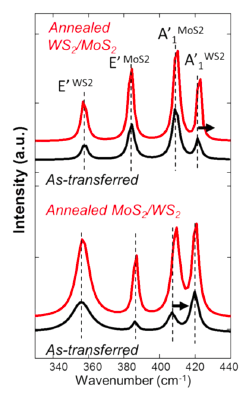
\includegraphics[scale=0.7]{Heterostructures/HeterostructureRamanSpectrumIntro.png}
		\caption{Heterostructure Raman spectrum}
		\label{fig:HeterostructureRamanSpectrumIntro}
	\end{center}
\end{figure}

\begin{figure}[h]
	\begin{center}
		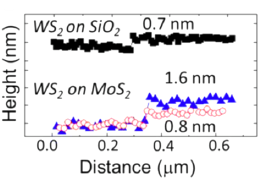
\includegraphics[scale=1]{Heterostructures/HeterostructureAFMProfile.png}
		\caption{Comparison of AFM profiles of $WS_2$ on $Si/SiO_2$ and $MoS_2$}
		\label{fig:HeterostructureAFMProfile}
	\end{center}
\end{figure}


\subsection{Photoluminescence}

\begin{figure}[h]
	\begin{center}
		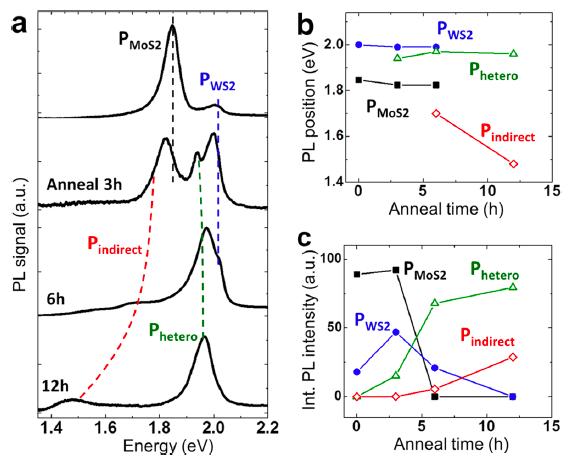
\includegraphics[scale=1]{Heterostructures/HeterostructurePLSpectrumIntro.png}
		\caption{PL Spectrum of heterostructure}
		\label{fig:HeterostructurePLSpectrumIntro}
	\end{center}
\end{figure}

The vertical heterostructures were further characterized by photoluminescence (PL) spectroscopy.
The as transferred heterostructures manifest PL peak typical of $MoS_2$ and $WS_2$. The spectrum can be defined as additive. The PL peak of $MoS_2$ show intensity much higher $WS_2$ and this was attributed to possibly higher density of defects in $WS_2$ associated with its higher growth temperatures. After annealing the $WS_2$/$MoS_2$ heterostructures, the PL spectrum gradually changes. The transition as seen in Figure \ref{fig:HeterostructurePLSpectrumIntro} from transferred to fully annealed bilayer heterostructures occur through the followings: (1) A new PL peak ($P_{hetero}$) appears at 1.94 eV, and its integrated intensity grows for prolonged annealing time. (2) Upon the annealing, $P_{MoS_2}$ and $P_{WS_2}$ gradually decrease up to the point of appearing as small features at lower and higher energy of the $P_{hetero}$ peak (3) at the end of 12 hours of annealing, another weak emission peak ($P_{indirect}$) appears at 1.75 eV, and the peak position rapidly and eventually red-shifts to ~1.5 eV. 

The explanation for this trend has been the following. As a consequence of the transfer the two monolayers end up well separated from each other due to residual water molecules and/or impurities trapped between the sheets. This large distance has been assessed by AFM (Figure \ref{fig:HeterostructureAFMProfile}). This system display PL peaks characteristics of isolated monolayer $MoS_2$ ($P_{MoS_2}$) and monolayer $WS_2$ ($P_{WS_2}$). After the annealing, the PL peak intensity of $MoS_2$ ($P_{MoS_2}$) and $WS_2$ ($P_{WS_2}$) decreases and two new peaks appear, called $P_{hetero}$ and $P_{indirect}$, with the former arising from the electronic coupling between the two monolayer materials while the latter arising due to the indirect band gap formed at the interface of the heterobilayer (Figure \ref{fig:HeterostructurePLSpectrumIntroComparison}). Because the $P_{indirect}$ peak position changes rapidly with the degree of coupling (annealing time). This has been attributed to a phonon-assisted, indirect bandgap transition, which involves the valence band maximum (VBM) at the {$\Gamma$}-point and the conduction band minimum (CBM) at the K-point. To prove this hypothesis, the authors have fabricated by transfer method a $MoS_2$/$MoS_2$ heterostructure and the indirect peak has similar behaviour. This suggested that the indirect peak can be associated with a similar behaviour as the bulk material. DFT calculations has supported this hypothesis \cite{Zande2014}. The formation of a type II heterojunction led to establishing a large electric field which develops across the ~1 nm thick junction. This leads to strong exciton splitting by which holes (electrons) are rapidly swept from $MoS_2$ to $WS_2$ (from $WS_2$  to $MoS_2$).

In order to understand the interlayer interactions DFT simulations have been performed. It has been observed that the twist angle between 2 layers has an effect on several properties of the TMDCs. By twisting the layers from being aligned at 0{\degree} to 30{\degree} the distance between the layers increases by about 0.3 \r{A}. The trend then reverses with distance returning back at 60 {\degree} to the same value as at the 0{\degree}. Additionally it has been predicted that as the twist angle changes from 0{\degree} to 30{\degree} the valence band at K point remains mostly unchanged while the valence band at $\Gamma$ point rises. Due to this the direct transition K-K remains unchanged while the indirect K-$\Gamma$ transition shows lower energy gap. As an explanation of that phenomenon it has been noted that the both valence and conduction band states at K point involve primarily $Mo$ states that are located within the layer. The valence state at the $\Gamma$ point however involves appreciable $p_z$ content of $S$ atoms and $Mo-d_z^2$. Because of that the overlap between those $p_z$ states of $S$ atoms varies significantly with the layer separation.

\begin{figure}[h]
	\begin{center}
		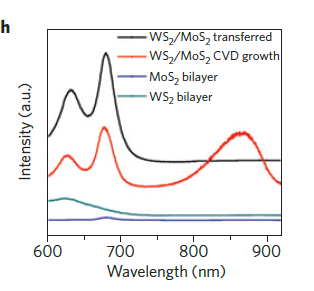
\includegraphics[scale=1]{Heterostructures/HeterostructurePLSpectrumIntroComparison.png}
		\caption{Comparison of PL spectra}
		\label{fig:HeterostructurePLSpectrumIntroComparison}
	\end{center}
\end{figure}

The CVD grown heterostructures shows a bandgap of 1.42 eV while at the same time separate pronounced PL peaks of $MoS_2$ and $WS_2$ can be seen (Figure \ref{fig:HeterostructurePLSpectrumInterlayerIntro} [].  
Subsequent studies have tremendously developed the understanding of the heterobilayer PL behaviour. The main factor which has been taken into consideration in the following studies is the mismatch angle between the lattices orientations of the two monolayers.
Experimentally, it was found that the twist angle in a heterobilayer determines the photoluminescence efficiency of interlayer excitons (bound  electrons and holes situated in adjacent layers) and their peak position.
It has been hypothesized that twist-angle-dependent interlayer orbital hybridization can cause the variation in the photon emission energies of indirect excitons in heterobilayers (e.g. $MoS_2$/$WSe_2$) and also in $MoS_2$ bilayers. Additional experimental work has reported similar results [][]. 

Specifically, in a study by Kunstamnn \cite{Kunstmann2018} the heterobilayer region of $MoS_2$/$WSe_2$ shows the peaks of the two individual materials are discernible among with a new peak near 1.6 eV. This has been interpreted as the indirect exciton, and renamed as interlayer exciton (ILE). By altering the twist angle between the $MoSe_2$ and $WSe_2$ layers from 0{\degree} to 30{\degree} the ILE peak intensity has decreased and further from 30{\degree} to 60{\degree} the intensity has increased again. Similarly the ILE peak position has blueshifted from 0{\degree} to 30{\degree} and redshifted back from 30{\degree} to 60{\degree}. The separation between the layers is also found to be highest at about 30{\degree} and smallest at 0{\degree} or 60{\degree}. At the same time the other PL peaks, associated with monolayer $WSe_2$ and $MoS_2$, are unaffected. The ILEs can be therefore associated with the K-$\Gamma$ transition.

\begin{figure}[h]
	\begin{center}
		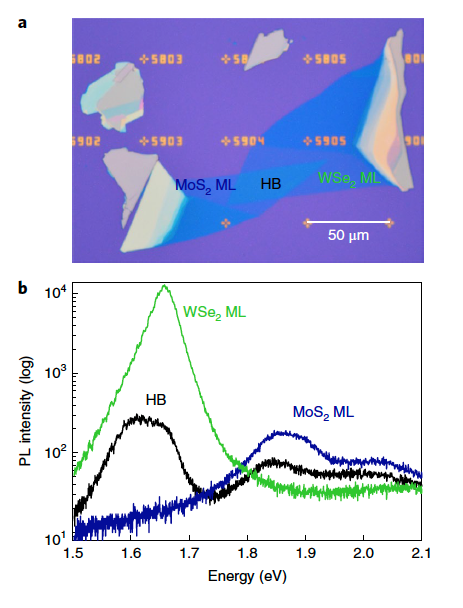
\includegraphics[scale=1]{Heterostructures/HeterostructurePLSpectrumInterlayerIntro.png}
		\caption{PL spectra taken from heterostructure \cite{Kunstmann2018}}
		\label{fig:HeterostructurePLSpectrumInterlayerIntro}
	\end{center}
\end{figure}

Very recently, Alexeev et al \cite{Alexeev2019} have shown the latest achievement in the field consist of bilayered TMDs heterostructures formed by transfer of CVD grown TMD as well as mechanically exfoliated. It has been shown that in the $WSe_2$/$MoS_2$ heterostructure the PL peak associated with $MoS_2$ monolayer redshifts while the one of the $WSe_2$ monolayer remains largely unaffected. Additionally as the twist between the layers increases from 0{\degree} to 60{\degree} the position of that PL peak increases initially and plateaus soon after and drops again near the 60{\degree} twist. It has been then suggested that a strong hybridazation takes place between interlayer and intralayer excitons. The Moir\'{e} pattern formed by twisting the layers results in formation of mini Brillouin zones. Those mini Brillouin zones (mBZ) at small angle twists result in additional interlayer peaks.  Those additional peaks are very strongly twist angle dependent and become less intense and more blueshifted at higher twist angles. 

\begin{figure}[h]
	\begin{center}
		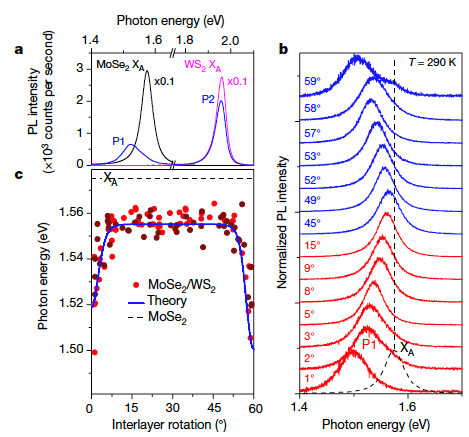
\includegraphics[scale=1]{Heterostructures/HeterostructurePLSpectrumInterlayerTwist.png}
		\caption{PL spectra of heterostructure \cite{Alexeev2019}}
		\label{fig:HeterostructurePLSpectrumInterlayerTwist}
	\end{center}
\end{figure}